\documentclass{article}
\usepackage[fleqn]{amsmath}
\DeclareMathOperator{\imp}{impulse(0)}

\usepackage{amssymb,cancel}
\usepackage{mathtools}

\usepackage{tikz,caption}
\tikzstyle{block}=[draw, minimum size=3.5em]
\tikzstyle{add}=[circle,draw]
\tikzstyle{arrow}=[thick,->,>=stealth]
\usetikzlibrary{shapes.geometric,arrows,positioning,calc}

\usepackage{titlesec, hyperref}
\newcommand{\sectionbreak}{\clearpage}
\newcommand{\R}{\mathbb{R}}

\let\OldPart\part
\renewcommand{\part}{\newpage\OldPart}

\title{Model Identification and Data Analysis}
\author{Matteo Secco}

\begin{document}
\maketitle
\newpage
\tableofcontents
\newpage

\part{Prediction}
\section{Probability Recall}

\subsection{Random Vectors}

\paragraph{Variance}
$Var[v]=E[(v-E[v])^2]$
\paragraph{Cross-Variance}
$Var[v,u]=E[(v-E[v])(u-E[u])]$
\paragraph{Variance Matrix}
$\begin{vmatrix}
	Var[v_1]			&	.	&	.	&	Var[v_1,v_k]		\\
		.			&	.	&		&		.			\\
		.			&		&	.	&		.			\\
	Var[v_k,v_1]		&	.	&	.	&	Var[v_k]			\\
				
\end{vmatrix}$
\paragraph{Covariance coefficient}
	$\delta[i,j]=\frac{Var[i,j]}{\sqrt{Var[i]}\sqrt{Var[j]}}$\\
	$\delta[i,j]=0 \implies$ i, j uncorrelated\\
	$\left|\delta[i,j]\right|=1 \implies i=\alpha j$
	
\subsection{Random processes} $v(t,s) |$ t time instant, s expetiment outcome (generally given)

\paragraph{Mean} $m(t)=E[v(t,s)]$
\paragraph{Variance}
$\lambda^2 (t)=Var[v(t)]$ 
\paragraph{Covariance function}
$\gamma(t_1,t_2)=E[(v(t_1)-m(t_1))(v(t_2)-m(t_2))]=\gamma(t_2,t_1)$
\paragraph{Normalized Covariance Function}
$\rho(\tau)=\frac{\gamma(\tau)}{\gamma(0)}$\\
$\forall$ stationary processes: $|\rho(\tau)|\leq1	\quad\forall\tau$

\subsection{Important process classes}

\paragraph{Stationary process}
\begin{itemize}
	\item $m(t)=m$ constant
	\item $\lambda^2 (t)=\lambda^2$ constant
	\item $\gamma(t_1,t_2)=f(t_2-t_1)=\gamma(\tau)$ covariance depends only on time difference $\tau$
\end{itemize}
$|\gamma(\tau)|\leq\gamma(0)		\quad\forall\tau$
\paragraph{White noise} $\eta(t)\sim WN(m,\lambda^2)$
\begin{itemize}
	\item Stationary process
	\item $\gamma(\tau)=0	\quad\forall\tau\neq0$
\end{itemize}
$v(t)=\alpha \eta (t)+\beta	\quad 
\eta (t)\sim WN(0,\lambda^2)	
\qquad\implies\qquad 
v(t)\sim WN(\beta,\alpha^2 \lambda^2)$

\section{Spectral Analysis}

\subsection{Foundamentals}
\paragraph{Spectrum} \[
\Gamma(\omega)=\overbrace{F(\gamma(\tau))}^\text{Fourier transform}=\sum_{\tau=-\infty}^{+\infty}\gamma(\tau)\cdot e^{-j\omega\tau}
\]
\paragraph{Euler formula} $\Gamma(\omega)=\gamma(0)+2cos(\omega)\gamma(1)+2cos(2\omega)\gamma(2)+...$
\paragraph{Spectrum properties} 
\begin{itemize}
	\item $\Gamma: \R \to \R$
	\item $\Gamma\text{ is periodic with }T=2\pi$
	\item $\Gamma\text{ is even }[\Gamma(-\omega)=\Gamma(\omega)]$
	\item $\Gamma(\omega)\geq 0 \quad \forall\omega$
\end{itemize}
$\eta(t) \sim WN(0,\lambda^2) \quad\implies\quad \Gamma_\eta(\omega)=\gamma(0)=Var[\eta(t)]=\lambda^2$
\paragraph{Anti-Transform}
\[
\gamma(\tau)=\frac{1}{2\pi}\int_{-\pi}^{+\pi} \Gamma(\omega)e^{k\omega\tau}\,dw
\]
\paragraph{Complex spectrum}
\[
\phi(z)=\sum_{\tau =-\infty}^{+\infty} \omega(\tau)z^{-\tau}
\]
\[
\Gamma(\omega)=\Phi(e^{j\omega})
\]

\subsection{Fundamental theorem of Spectral Analysis} 

\paragraph{Fundamental theorem of Spectral Analysis} allows to derive the (real and/or complex) spectrum of the output from  the input and the transfer function of the system

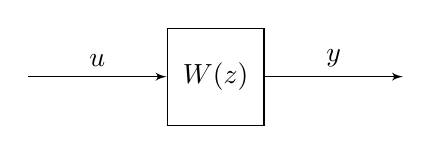
\begin{tikzpicture}[node distance=5em,auto,>=latex']
    \node [block] (W) {$W(z)$};
    \node (u) [left=of W, coordinate] {};
    \node [coordinate] (y) [right=of W]{};
    \path[->] (u) edge node {$u$} (W);
    \path[->] (W) edge node {$y$} (y);
\end{tikzpicture}

\begin{alignat*}{2}
	\Gamma_{yy}(\omega)&=|W(e^{j\omega})|^2 & \cdot \Gamma_{uu}(\omega)\\
	\Phi_{yy}(z)&=W(z)W(z^{-1})				& \cdot \Phi_{uu}(z)
\end{alignat*}

\subsection{Canonical representation of a Stationary Process}
A stationary process can be represented by an infinite number of transfer functions. The canonical representation is the transfer function $W(z)$ such that:
\begin{itemize}
\item Numerator and denominator have \underline{same degree}
\item Numerator and denominator are \underline{monic} (highest grade coefficient is 1)
\item Numerator and denominator are \underline{coprime} ($W(z)$ cannot be simplified)
\item numerator and denominator are \underline{stable polynomials} (all poles and zeros of $W(z)$ are inside the unit disk)
\end{itemize}

\section{Moving Average Processes}
Given $\eta(t) \sim WN(0,\lambda^2)$
\subsection{MA(1): }
\paragraph{Model}
\[v(t)=c_0\eta(t)+c_1\eta(t-1)\]


\subparagraph{Mean}
\begin{alignat*}{2}
	E[v(t)]		&=	c_0\cdot E[\eta(t)]	&	&+	c_1\cdot E[\eta(t)]	\\
				&=	c_0\cdot 0			&	&+	c_1\cdot 0			\\
	\Aboxed{E[v(t)]&=0}
\end{alignat*}


\subparagraph{Variance}
\begin{alignat*}{3}
	Var[v(t)]	&=	E[(v(t)	\underbrace{-E[v(t)])^2}_{0}]													\\
				&=	E[(v(t))^2]						\\
				&=	E[(c_0\cdot	\eta(t)^2		&+&	c_1\cdot	\eta(t-1))^2]	\\
				&=	c_0^2\cdot 	E[\eta(t)^2]		&+&	c_1^2\cdot E[\eta(t-1)^2]	&+	\underbrace{2 c_0 c_1 \cdot E[\eta(t)\eta(t-1)]}_0\\
				&=	c_0^2\cdot 	E[\eta(t)^2]		&+&	c_1^2\cdot E[\eta(t-1)^2]\\
				&=	c_0^2\lambda^2				&+&	c_1^2\lambda^2\\
	\Aboxed{Var[v(t)]&=(c_0^2+c_1^2)\lambda^2}
\end{alignat*}


\subparagraph{Covariance}
\begin{alignat*}{4}
	\gamma(t_1,t_2)	&=	E[(v(t_1)-E[v(t_1)])				&\cdot 	&		(v(t_2)-E[v(t_2)])]\\
					&=	E[(c_0\eta(t_1)+c_1\eta(t_1-1))	&\cdot 	&		(c_0\eta(t_2)+c_1\eta(t_2-1))]\\
					&=	c_0^2E[\eta(t_1)\eta(t_2)]		&+&				c_1^2E[\eta(t_1-1)\eta(t_2-1)\\
					&									&+&				c_0c_1E[\eta(t_1)\eta(t_2-1)]
						+c_0c_1E[\eta(t_1-1)\eta(t_2)]
\end{alignat*}
\[
\boxed{
	\gamma(\tau)=\begin{cases}
		c_0^2\lambda^2+c_1^2\lambda^2	&\text{if }\tau=0\\
		c_0c_1\lambda^2					&\text{if }\tau=\pm 1\\
		0								&\text{otherwise}
	\end{cases}
}
\]

\subsection{MA(n)}

\paragraph{Model}
\begin{align*}
v(t)&=c_0\eta(t)+c_1\eta(t-1)+...+c_n\eta(t-n)\\
&=(c_0+c_1z^{-1}+...+c_nz^{-n})\eta(t)
\end{align*}

\paragraph{Transfer function}
\[W(z)
=c_0+c_1z^{-1}+...+c_nz^{-n}
=\frac{c_0z^n+c_1z^{n-1}+...+c_n}{z^n}
\]\\
All poles are in the complex origin

\paragraph{Mean}
\begin{alignat*}{2}
E[v(t)]&=(c_0+c_1+...+c_n)\underbrace{E[\eta(t)]}_0\\
\Aboxed{E[v(t)&=0}
\end{alignat*}

\paragraph{Covariance function}
\[
\boxed{
\gamma(\tau)=
\begin{cases}
\lambda^2\cdot \sum_{i=0}^{n-\tau} c_ic_{i-\tau}	&	|\tau|\leq n\\
0	& \text{otherwise}
\end{cases}
}
\]
\subparagraph{example}
\begin{align*}
\gamma(0)&=(c_0^2+c_1^2+...+c_n^2)\lambda^2\\
\gamma(1)&=(c_0c_1+c_1c_2+...+c_{n-1}c_n)\lambda^2\\
\gamma(2)&=(c_0c_2+c_1c_3+...+c_{n-2}c_n)\lambda^2\\
&...\\
\lambda(n)&=(c_0c_n)\lambda^2\\
\lambda(k)&=0\:\forall k>n
\end{align*}

\subsection{MA($\infty$)}
\paragraph{Model}
\[
v(t)=c_0\eta(t)+c_1\eta(t-1)+...+c_k\eta(t-k)+...=\sum_{i=0}^{\infty}c_i\eta(t-i)
\]
\paragraph{Variance}
\[
\gamma(0)
=(c_0^2+c_1^2+...+c_k^2+...) \lambda^2
=\lambda^2 \sum_{i=0}^{\infty} c_i^2
\]
\subsection{Well definition of an MA($\infty$)}
We need to have $|\gamma(\tau)|\leq \gamma(0)$, so we must require that \\
$\boxed{ \gamma(0)=\lambda^2 \sum_{i=0}^{\infty} c_i^2 \text{ is finite}}$

\section{Auto Regressive Processes}
\subsection{AR(1)}
\paragraph{Model}
\[v(t)=av(t-1)+\eta(t)\]
\paragraph{Mean}
\begin{alignat*}{2}
E[v(t)]&=E[av(t-1)]+\overbrace{E[\eta(t)]}^0\\
&=aE[v(t-1)]\\
&=aE[v(t)]\\
(1-a)E[v(t)]&=0\\
\Aboxed{
E[v(t)]&=0
}
\end{alignat*}
\paragraph{Covariance}
\subparagraph{MA($\infty$) method}
Observe as an AR(1) can  be axpressed as an MA($\infty$)
\begin{align*}
v(t)
&=av(t-1)	&+&		\eta(t)\\
&=a[av(t-2)+\eta(t-1)]	&+&	\eta(t)\\
&=a^2v(t-2)				&+&	a\eta(t-1) + \eta(t)\\
&=a^2[v(t-3)+\eta(t-2)]	&+& a\eta(t-1) + \eta(t)\\
&=\underbrace{a^nv(t-n)}_{\to 0}+ \underbrace{\sum_{i=0}^\infty a^i\eta(t-i)}_{\text{MA($\infty$)}}
\end{align*}
In particular, the result depends on an $MA(\infty)$ having $\sum_{i=0}^{\infty} c_i = \sum_{i=0}^{\infty} a^i$.\\
To check if the variance is finite we check $\gamma(0)=\lambda^2 \sum_{i=0}^{\infty} a^{2i}<\infty$. The given is a geometric series, convergent for $|a|<1$. Under this hypothesis its value is
\[
\gamma(0)=\lambda^2 \sum_{i=0}^{\infty} a^{2i}=\frac{\lambda^2}{1-a^2}
\] 
Applying the formula of the variance of MA processes we get\\
\hspace*{-1cm}\vbox{	%slightly move these equations to the right
 
 \begin{alignat*}{7}
\gamma(1)
	&=(c_0c_1+c_1c_2+...)\lambda^2
	&=(a+aa^2+...)\lambda^2
	&=a(1+a^2+a^4+...)\lambda^2
	&=a\lambda^2\sum_{i=0}^{\infty} a^{2i}
	&=a\frac{\lambda^2}{1-a^2}
	&=a\gamma(0)\\
\gamma(2)
	&=(c_0c_2+c_1c_3+...)\lambda^2
	&=(a^2+aa^3+...)\lambda^2
	&=a^2(1+a^2+a^4+...)\lambda^2
	&=a^2\lambda^2\sum_{i=0}^{\infty} a^{2i}
	&=a^2\frac{\lambda^2}{1-a^2}
	&=a^2\gamma(0)\\
\Aboxed{
\gamma(\tau)&=a^{|\tau|}\frac{\lambda^2}{1-a^2}
}
\end{alignat*}
} 
\subparagraph{Yule-Walkler Equations}
\begin{align*}
Var[v(t)]	
	&=E[v(t)^2]\\
	&=E[(av(t)+\eta(t))^2]\\
	&=a^2\underbrace{E[v(t-1)^2]}_{\substack{=Var[v(t-1)]\\=Var[v(t)]\\=\gamma(0)}}
		+\underbrace{E[\eta(t)^2]}_{=\lambda^2}
		+2a \underbrace{E[v(t-1)\eta(t)]}_{
					\substack{	v(t-1)\text{ depends on } \eta(t-2)\\
								\eta(t)\text{ independent of }\eta(t-2)\\
								\implies\\
								E[v(t-1)\eta(t)]=0\\
								}}\\
\gamma(0)&=a^2\gamma(0)+\lambda^2\\
\Aboxed{
\gamma(0)&=\frac{\lambda^2}{1-a^2}
}
\end{align*}
To find $\gamma(\tau)$, we start from the model $v(t)=av(t-1)+\eta(t)$.
\begin{alignat*}{4}
v(t)&=av(t-1)&+&\eta(t)\\
v(t)v(t-\tau)&=av(t-1)v(t-\tau)&+&\eta(t)v(t-\tau)\\
\underbrace{E[v(t)v(t-\tau)]}_{\gamma(\tau)}&=
	a\underbrace{E[v(t-1)v(t-\tau)]}_{\gamma(\tau-1)}&+&
	\underbrace{E[\eta(t)v(t-\tau)]}_0\\
\Aboxed{
\gamma(\tau)&=a\gamma(\tau-1)
}
\end{alignat*}
We can join the two by inductive reasoning, obtaining
\[\boxed{
\gamma(\tau)=a^{|\tau|}\frac{\lambda^2}{1-a^2}
}\]
\subparagraph{Long Division} Leads to same result, but is boring

\subsection{AR(n)}
\paragraph{Model}
\[
v(t)=a_1v(t-1)+a_2v(t-2)+...+a_nv(t-n)+\eta(t)
\]
\paragraph{Transfer function}
\[
W(z)=\frac{z^n}{z^n-a_1z_{n-1}-...-a_n}
\]
\paragraph{Mean}
\begin{alignat*}{6}
E[v(t)]	&=	a_1E[v(t-1])	&+&a_2E[v(t-2)]	&+&...	&+&a_nE[v(t-n)]	&+&\underbrace{E[\eta(t)]}_0\\
m		&=	a_1m			&+&a_2m			&+&...	&+&a_nm\\
(1-a_1-a_2-...-a_n)m&=0\\
\Aboxed{
E[v(t)]&=0
}
\end{alignat*}
\section{ARMA Processes}
\paragraph{Model}
\[
v(t)=
	a_1v(t-1)+...+a_{n_a}v(t-n_a)+
	c_0\eta(t)+...+c_{n_c}v(t-n_c)
\]
Can also be espressed as $V(t)=\frac{C(z)}{A(z)}\eta(t)$, where
\begin{align*}
C(z)&=c_0+c_1z^{-1}+...+c_{n_c}z^{-n_c}\\
A(z)&=1-a_1z^{-1}-...-a_{n_a}z^{-n_a}
\end{align*}
Such process is stationary if all the poles of $W(z)$ are inside the unit disk.

\section{Prediction problem}
We want to predict $v(t+r)$ from $v(t), v(t-1), ...$, where $r$ is called prediction horizon, of the following stationary process:

\tikzstyle{block}=[draw, minimum size=3.5em]

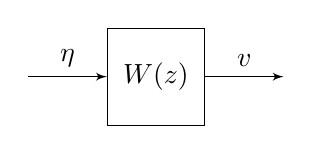
\begin{tikzpicture}[node distance=1cm,auto,>=latex']
    \node [block] (W) {$W(z)$};
    \node (wn) [left=of W, coordinate] {};
    \node [coordinate] (v) [right=of W]{};
    \path[->] (wn) edge node {$\eta$} (W);
    \path[->] (W) edge node {$v$} (v);
\end{tikzpicture}

\subsection{Fake problem}
Having a process with transfer function $W(z)$, we can compute it in polynomial form using the long division algorithm
\[
W(z)=w_0+w_1z^{-1}+w_2z^{-2}+...
\]
We can calculate
\[
v(t+r)=W(z)\eta(t+r)
= \underbrace{w_0 \eta(t+r)+w_1 \eta(t+r-1)+...+w_{r-1} \eta(t+1)}_{\alpha(t)\textbf{ unpredictable: }\text{future of }\eta\text{ involved}}
+ \underbrace{w_r \eta(t)+w_{r+1} \eta(t-1)+...}_{\beta(t) \textbf{ predictable}}
\]
The optimal fake predictor is then
\[
\boxed{
v(t+r|t)=w_r \eta(t)+w_{r+1}\eta(t-1)+...
}=\beta(t)
\]
And the prediction error is
\begin{align*}
\epsilon(t)&=v(t+r)&-&\hat{v}(t+r|t)\\
&= \alpha(t)+\beta(t)&-&\beta(t)\\
&=\alpha(t)\\
\end{align*}
\[
\boxed{
\epsilon(t)=w_0 \eta(t+r)+w_1 \eta(t+r-1)+...+w_{r-1} \eta(t+1)
}
\]
\[
\boxed{
Var[\epsilon(t)]=(w_0^2+w_1^2+...+w_{r-1}^2)\lambda^2
}
\]
\subsection{True Problem}
We want to estimate $v(t+r)$ form $v(t)$, having transfer function $W(z)$ and $\hat{W}_r(z)$ the solution to the fake problem. We can calculate the transfer function of the real predictor from the process as 
\[
\boxed{
W_r(z)=W(z)^{-1} \cdot \hat{W}_r(z)
}
\]
For ARMA processes a shortcut exists:
\[
\hat{v}_{\text{ARMA}}(t|t-1)=\frac{C(z)A(z)}{C(z)}
\qquad \text{having } W(z)=\frac{C(z)}{A(z)}
\]
\subsection{Prediction with eXogenous variables}
An exogenous variable is a \underline{deterministic} input variable in the system
\subsubsection{ARX model}
\begin{align*}
v(t)&=a_1v(t-1)+...+a_{n_a}v(t-n_a)+b_1u(t-1)+...+b_{n_b}u(t-n_b)+\eta(t)
A(z)v(t)&=B(z)u(t-1)+\eta(t)
\end{align*}
\paragraph{Transfer functions from u and $\eta$}
\[
W_u(z)=\frac{B(z)}{A(z)}\\
W_{\eta}(z)=\frac{1}{A(z)}
\]
\subsubsection{ARMAX model}
\begin{align*}
A(z)v(t)&=C(z)\eta(t)+B(z)u(t-1)\\
y(t)&=W(z)\eta(t)+G(z)u(t)
\end{align*}
\paragraph{Predictor}
\[
\hat{y}(t|t-1)=
\frac{C(z)-A(z)}{C(z)}y(t)
+\frac{B(z)}{C(z)}u(t-1)
\]

\newpage
\part{Identification}
Consists of estimating a model from data.
\section{Prediction Error Minimization} Aims to minimize $\epsilon(t)=v(t)-\hat{v}(t|t-r)$\\
Steps:
\begin{enumerate}
\item \textbf{Data collection:} collect $\vec{u}$ and $\vec{y}$
\item \textbf{Family selection:} choose a family of models $M(\theta)$
	\begin{description}
	\item[MA(1)] $\theta=[a]$
	\item[MA(n)] $\theta=[a_1,...,a_n]$
	\item[ARMA($n_a,n_c$)] $\theta=[a_1,...,a_{n_a},
	c_1,...,c_{n_c}]$
	\item[...]
	\end{description}
\item \textbf{Select an optimization criterion}
	\begin{description}
	\item[Mean Squared error] $J(\theta)=\frac{1}{N}\sum_{t=1}^N \epsilon_\theta(t)^2$
	\item[Mean absolute error] $J(\theta)=\frac{1}{N}\sum_{t=1}^N |\epsilon_\theta(t)|$
	\item[...]
	\end{description}
\item  \textbf{Optimization} find $\hat{\theta}=argmin\,J(\theta)\implies \frac{dJ(\theta)}{d\theta}=0$
\item \textbf{Validation} verify if the result satisfies the requirements
\end{enumerate}

\newpage
\appendix

\newpage
\part{Black-Box non-parametric I/O systems}
\section{State-space models}
\begin{center}
\begin{tikzpicture}[node distance=1cm,auto,>=latex']
    \node [block] (sys) {system};
    \node (u) [left=of sys] {$u(t)$};
    \node (y) [right=of sys]{$y(t)$};
    \node (d) [above=of sys]{$d(t)$};
    \path[->]
    		(u) edge (sys)
    		(sys) edge (y)
    		(d) edge[dotted] (sys);
\end{tikzpicture}
\end{center}
\paragraph{Known (measured) data}
\begin{align*}
&\{u(1),\dots,u(N)\}&\text{input}\\
&\{y(1),\dots,y(N)\}&\text{output}\\
\end{align*}
\subsection{State-space representation}
\[
\begin{cases}
x(t+1)=Fx(t)+Gu(t)&\quad\text{state equations}\\
y(t)=Hx(t)+Du(t)&\quad\text{output equations}
\end{cases}
\]
Where $F_{n\times n}$, $G_{n\times 1}$, $H_{1\times n}$ and $D_{1\times 1}$ are matrices.
\paragraph{S.S. representation is not unique} Given any invertible matrix $T$, let $F_1=TFT^{-1}$, $G_1=TG$, $H_1=HT^{-1}$, $D_1=D$. Then the system $\{F,G,H,D\}$ is equivalent to the system $\{F_1,G_1,H_1,D_1\}$.
\subsection{Transfer function representation}
\[
W(z)
=
\frac{B(z)}{A(z)}z^{-k}
=
\frac{
	b_0+b_1z^{-1}+\dots+b_pz^{-p}
}{
	a_0+a_1z^{-1}+\dots+a_nz^{-n}
}z^{-k}
\]
$W(z)$ is a rational function of the $z$ operator $\rightarrow$ is a digital filter
\paragraph{Infinite impulse response} 
$W(z)=
\frac{
	z^{-1}
}{
	1+\frac{1}{3}z^{-1}
}$
\paragraph{Finite impulse response}
$
W(z)=z^{-1}+\frac{1}{2}z^{-2}+\frac{1}{4}z^{-3}
$

\subsection{Convolution of the input with the inpulse response}
Let's call $\omega(1), \omega(2), \dots$ the values of $y(t)$ when $u(t)=\imp$, and let's measure the values of $y$ at different times: . Then it can be proven that for any $u(t)$
\[
y(t)=\sum_{k=0}^\infty \omega(k)u(t-k)
\]

\section{Converting representations one to another}
\subsection{State space to Transfer function}
Consider a strictly propter system:
\[
\begin{cases}
x(t+1)=Fx(t)+Gu(t)\\
y(t+1)=Hx(t)+\cancelto{0}{Du(t)}
\end{cases}
\Rightarrow
\begin{cases}
x(t+1)=Fx(t)+Gu(t)\\
y(t)=Hx(t)
\end{cases}
\]
Applying the $z$ operator we get
\begin{align*}
zx(t)&=Fx(t)+Gu(t)\\
x(t)(zI-F)&=Gu(t)\\
x(t)&=(zI-F)^{-1}Gu(t)\\
y(t)&=H(zI-F)^{-1}Gu(t)
\end{align*}
And we can extract the transfer function:
\[
W(z)=H(zI-F)^{-1}G
\]

\subsection{Transfer Function to State Space}
We have the transfer function
\[
W(z)=\frac{b_0z^{n-1}+b_1z^{n-2}+\dots+b_{n-1}}{z^n+a_0z^{n-1}+\dots+a_n}
\]
The formulas for the state space matrices is
\[
F=
\begin{bmatrix}
0&1&0&\dots&0\\
0&0&1&\ddots&\vdots\\
\vdots&\vdots&\ddots&\ddots&0\\
0&0&\dots&0&1\\
-a_n&-a_{n-1}&\dots&\dots&-a_1
\end{bmatrix}
\quad
G=\begin{bmatrix}
0\\0\\\vdots\\0\\1
\end{bmatrix}
\quad
H=\begin{bmatrix}
b_{n-1}&b_{n-2}&\dots&b_0
\end{bmatrix}
\quad
D=0
\]

\subsection{Transfer function to Impulse response}
Obtained by computing the $\infty$ long division of $W(z)$

\subsection{Impulse response to Tranfer function}
\paragraph{Z-transform} Given a discrete-time signal $s(t)$ such that $\forall t<0:s(t)=0$, it's Z-transform is
\[
\mathcal{Z}=\sum_{t=0}^\infty s(t)z^{-t}
\]
It can be proven that:
\[
W(z)=\mathcal{Z}(\omega(t))=\sum_{t=0}^\infty \omega(t)z^{-1}
\]
NB: this works only in theory because of the infinite sum

\subsection{State space to Impulse response}
Consider the state space model:
\[
\begin{cases}
x(t+1)=Fx(t)+Gu(t)\\
y(t)=Hx(t)
\end{cases}
\]
We have that:
\begin{align*}
x(1)&=\cancelto{0}{Fx(0)}+Gu(0)&=Gu(0)\\
y(1)&=Hx(1)&=HGu(0)\\
\\
x(2)&=Fx(1)+Gu(1)&=FGu(0)+Gu(1)\\
y(2)&=Hx(2)&=HFGu(0)+HG(u1)\\
\\
x(3)&=Fx(2)+Gu(2)&=F^2Gu(0)+FGu(1)+Gu(2)\\
y(3)&=Hx(3)&=HF^2Gu(0)+HFGu(1)+HGu(2)\\
\vdots
\end{align*}
\[
y(t)=0u(t)+HGu(t-1)+HFGu(t-2)+HF^2Gu(t-3)+\dots
\]
The IR is:
\[
\omega(t)=
\begin{cases}
0 & \text{if } t=0\\
HF^{t-1}G & \text{if } t>0
\end{cases}
\]


\section{Controllability and Observability}
\[
\begin{cases}
x(t+1)=Fx(t)+Gu(t)\\
y(t)=Hx(t)
\end{cases}
\]
\paragraph{Fully observable system} The system is fully observable (from the output) $\iff$ the observability matrix is full rank:
\[
O=\begin{bmatrix}
H\\HF\\\vdots\\HF^{n-1}
\end{bmatrix}
\qquad
rank(O)=n
\]
\paragraph{Fully controllable system} The system is fully controllable (from the input) $\iff$ the controllability (also called reachability) matrix is full rank:
\[
R=\begin{bmatrix}
G&FG&\dots&F^{n-1}G
\end{bmatrix}
\qquad
rank(R)=n
\]

\section{Hankel Matrix}
Starting from $\omega(1),\omega(2),\dots,\omega(N)$ where $N\geq 2n-1$, we can build the Hankel Matrix of order $n$:
\[
H_n=\begin{bmatrix}
\omega(1)&\omega(2)&\omega(3)&\dots&\omega(n)\\
\omega(2)&\omega(3)&\omega(4)&\dots&\omega(n+1)\\
\omega(3)&\omega(4)&\omega(5)&\dots&\omega(n+2)\\
\vdots&\vdots&\vdots&\ddots&\vdots\\
\omega(n)&\omega(n+1)&\omega(n+2)&\dots&\omega(2n-1)\\
\end{bmatrix}
\]
Knowing that
\[
\omega(t)=
\begin{cases}
0&\text{if }t=0\\
HF^{t-1}G&\text{if }t>0
\end{cases}
\]
We can rewrite
\[
H_n=
\begin{bmatrix}
HG&HFG&HF^2G&\dots&HF^{n-1}G\\
\vdots&\ddots&&&\vdots\\
\vdots&&\ddots&&\vdots\\
\vdots&&&\ddots&\vdots\\
HF^{n-1}G&\dots&\dots&\dots&HF^{2n-2}G
\end{bmatrix}
=
\begin{bmatrix}
H\\HF\\\vdots\\HF^{n-1}
\end{bmatrix}
\cdot
\begin{bmatrix}
G&FG&\dots&F^{n-1}G
\end{bmatrix}
=
O\cdot R
\]

\section{Subspace-based State Space System Identification}
\paragraph{Impulse experiment} Measure $y(t)$ under the input $u(t)=\imp (0)$\\
How to derive $F,G,H$ from $\omega(0),\dots,\omega(n)$?
\begin{itemize}
\item Assuming the IR measurement to be noise free $\rightarrow$ easier, not realistic
\item Measure $\hat{\omega(t)}$ as a noisy signal and compute $\omega(t)=\eta(t)-\hat{\omega}(t)$
\end{itemize}

\subsection{Obtain $F,G,H$ from a noise-free IR}
\begin{enumerate}
\item
	Build the Hankel matrix of increasing order, and conpute the rank until $rank(H_n)=rank(H_{n+1})$. Then, $n$ is the order of the IR
	\[
	H_1=\begin{bmatrix}
	\omega(1)
	\end{bmatrix}
	\quad
	H_2=\begin{bmatrix}
	\omega(1)&\omega(2)\\
	\omega(2)&\omega(3)
	\end{bmatrix}
	\quad
	H_3=\dots
	\quad
	\dots
	\quad
	H_n=\dots
	\]
\item Take $H_{n+1}$ and factorize it in two rectangular matrix of size $(n+1)\times n$ and $n\times (n+1)$: $H_{n+1}=O_{n+1}\cdot R_{n+1}$, where
	\[
	O_{n+1}=\begin{bmatrix}
	H\\HF\\\vdots\\HF^n
	\end{bmatrix}
	\qquad
	R_{n+1}=\begin{bmatrix}
	G&FG&\dots&F^nG
	\end{bmatrix}
	\]
\item Estimate H,F,G:
	\begin{itemize}
	\item Extract F and G from the first element of O and R
	\item Define:
	\[
	O_1=\begin{bmatrix}
	H\\HF\\\vdots\\HF^{n-1}
	\end{bmatrix}
	\qquad
	O_2=\begin{bmatrix}
	HF\\\vdots\\HF^n
	\end{bmatrix}\\
	\]
	\item Observe that $O_1F=O_2$, so $F=O_1^{-1}O_2$
	\end{itemize}	
\end{enumerate}

\section{Obtain $F,G,H$ from a noisy IR}
The measurement is of $\hat{\omega}(t)=\omega(t)+\eta(t)$. To identify the process:
\begin{enumerate}
\item Build the Hankel matrix from data using all the $N$ data available in one shot:
\[
\hat{H}_{q \times d}=
\begin{bmatrix}
\hat{\omega}(1)&\hat{\omega}(2)&\dots&\hat{\omega}(d)\\
\hat{\omega}(2)&\hat{\omega}(3)&\dots&\hat{\omega}(d+1)\\
\vdots&\vdots&\ddots&\vdots\\
\hat{\omega}(q)&\hat{\omega}(q+1)&\dots&\hat{\omega}(q+d+1)\\
\end{bmatrix}
\]
Where $q+d+1=N$
\item Calculate the Singular Value Decomposition of $\hat{H}_{q \times d}$:
\[
\hat{H}_{q \times d}=\hat{U}_{q \times q} \cdot \hat{S}_{q \times d} \cdot \hat{V}^T_{d \times d}
\]
$\hat{U}$ and $\hat{V}$ are unitary matrices: they are invertible and their inverses are equal to their transpose.
\[
\hat{S}=\begin{bmatrix}
\sigma_1\\
&\sigma_2\\
&&\ddots\\
&&&\sigma_d
\end{bmatrix}
\]
\item Plot the singular values ($\sigma_i$)and cut-off the three matrices:
	\begin{itemize}
	\item Ideally, after a certain $n$ (the order of the IR) there would be a jump dividing the signal (before) from the noise (after)
	\item In reality no clear distinction exists, but it's possible to identify an interval of possible values of $n$. A tradeoff between complexity, precision and oferfitting takes place
	\end{itemize}
\item Split $\hat{U},\hat{S},\hat{V}^T$ obtaining $U_{q \times n}$, $S_{n \times n}$, $V^T_{n \times d}$ and then recreate $H_{qd}=USV^T$
\item $H$ and $G$ are estimated as for the unnoisy case. To estimate $F$ we can build $O_1$ and $O_2$ as before, but then the system $O_1 \cdot F = O_2$ cannot be solved directly as $O_1$ is not square. We can instead compute the approximate least-square solution of the system:
\[
F=(O_1^TO_1)^{-1}O_1^TO_2
\]
\end{enumerate}

\part{Parametric black-box system identification using frequency-domain approach}
\section{Experiment design and data pre-processing}
\begin{enumerate}
\item Select a set of excitation frequencies $\{\omega_1,\dots,\omega_H\}$. Usually $\omega_i-\omega_{i-1}$ is constant $\forall i \in \{2,\dots,H\}$. $\omega_H$ must be selected according to the bandwidth of the system
\item Make $H$ independent experiments:
\begin{figure}[h]
\centering
\captionsetup{labelformat=empty}
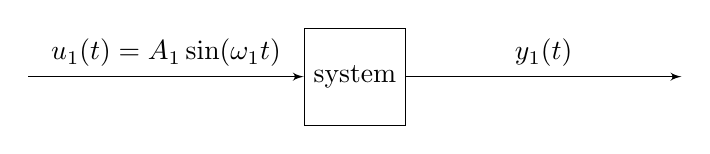
\begin{tikzpicture}[node distance=3.5cm,auto,>=latex']
    \node [block] (sys) {system};
    \node (u) [left=of sys, coordinate] {};
    \node (y) [right=of sys,coordinate]{};
    \path[->]
    		(u) edge node{$u_1(t)=A_1\sin(\omega_1t)$} (sys)
    		(sys) edge node{$y_1(t)$} (y);
\end{tikzpicture}
\caption{Experiment 1}
\bigskip
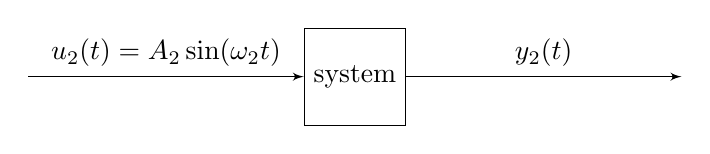
\begin{tikzpicture}[node distance=3.5cm,auto,>=latex']
    \node [block] (sys) {system};
    \node (u) [left=of sys, coordinate] {};
    \node (y) [right=of sys,coordinate]{};
    \path[->]
    		(u) edge node{$u_2(t)=A_2\sin(\omega_2t)$} (sys)
    		(sys) edge node{$y_2(t)$} (y);
\end{tikzpicture}
\caption{Experiment 2}
\caption{\vdots}
\bigskip
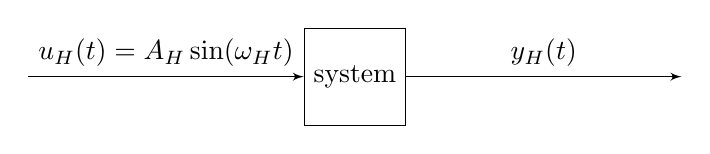
\begin{tikzpicture}[node distance=3.5cm,auto,>=latex']
    \node [block] (sys) {system};
    \node (u) [left=of sys, coordinate] {};
    \node (y) [right=of sys,coordinate]{};
    \path[->]
    		(u) edge node{$u_H(t)=A_H\sin(\omega_Ht)$} (sys)
    		(sys) edge node{$y_H(t)$} (y);
\end{tikzpicture}
\caption{Experiment H}
\end{figure}
\item Focusing on experiment $i$, because of noise the real value of the output will be (unknowns are underlined)
\[
\hat{y_i}=
\underline{B_i}\sin(\omega_it+\underline{\phi_i})=
\underline{a_i}\sin(\omega_it)+\underline{b_i}\cos(\omega_it)
\]
Using the second equation (since it is linear in the unknowns). We want to determine
\[
\{\hat{a_i},\hat{b_i}\}=\arg\min_{\{a_i,b_i\}} J_N(a_i,b_i)
\]
\[
J_N(a_i,b_i)=\frac{1}{N}\sum_{t=1}^{N} \left( 
\underbrace{
	y_i(t)
}_{
	\text{measurement}
}
\underbrace{
	-a_i\sin(\omega_it)
	-b_i\cos(\omega_it)
}_{
	\text{model output}
}
\right)^2
\]
This can be solved explicitly
\begin{align*}
\frac{\delta J_N}{\delta a_i}&=
\frac{2}{N}\sum_{t=1}^N
\left(-\sin(\omega_it)\right)
\left(y_i(t)-a_i\sin(\omega_it)-b_i\cos(\omega_it)\right)&=0\\
\frac{\delta J_N}{\delta b_i}&=
\frac{2}{N}\sum_{t=1}^N
\left(-\cos(\omega_it)\right)
\left(y_i(t)-a_i\sin(\omega_it)-b_i\cos(\omega_it)\right)&=0
\end{align*}
Which results in the following linear system:
\[
\begin{bmatrix}
\sum_{t=1}^N \sin(\omega_it)^2
&
\sum_{t=1}^N \sin(\omega_it)\cos(\omega_it)
\\
\sum_{t=1}^N \sin(\omega_it)\cos(\omega_it)
&
\sum_{t=1}^N \cos(\omega_it)^2
\end{bmatrix}
\begin{bmatrix}
a_i\\b_i
\end{bmatrix}
=
\begin{bmatrix}
\sum_{t=1}^N y_i(t)\sin(\omega_it)
\\
\sum_{t=1}^N y_i(t)\cos(\omega_it)
\end{bmatrix}
\]
\item We want to move back to sin-only form:
\begin{align*}
\hat{\phi_i}&=\arctan \left(\frac{\hat{b_i}}{\hat{a_i}}\right)\\
\hat{B_i}&=\frac{\frac{\hat{a_i}}{\cos\hat{\phi_i}}+\frac{\hat{b_i}}{\sin\hat{\phi_i}}}{2}
\end{align*}
\item Repeating H experiments we obtain
\begin{align*}
\{\hat{B_1},\hat{\phi_1}\} &\Rightarrow \frac{\hat{B_1}}{A_1}e^{j\hat{\phi_1}}\\
&\vdots\\
\{\hat{B_H},\hat{\phi_H}\} &\Rightarrow \frac{\hat{B_H}}{A_H}e^{j\hat{\phi_H}}\\
\end{align*}
So we have H complex numbers representing the frequency response of $W(z)$. These numbers are our dataset
\end{enumerate}
\section{Model class selection}
\[
\mathcal{M(\theta)}:
W(z,\theta)=
\frac{b_0+b_1z^{-1}+\dots+b_pz^{-p}}{1+a_1z^{-1}+\dots+a_nz^{-n}}
z^{-1}
\qquad
\theta=\begin{bmatrix}
a_1\\\vdots\\a_n\\b_0\\\vdots\\b_p
\end{bmatrix}
\]
\section{Performance index}
\[
J_H(\theta)=
\frac{1}{H}
\sum_{i=1}^H
\left(
W(e^{j\omega_i},\theta)
-
\frac{\hat{B_i}}{A_i}e^{j\hat{\phi_i}}
\right)^2
\]
\section{Optimization}
\[
\hat{\theta}=\arg \min_\theta J_H(\theta)
\]

\part{Kalman filter}
Based on SS representation:
\[
\begin{cases}
x(t+1)=Fx(t)+Gu(t)+v_1(t)&v_1\sim WN\\
y(t)=Hx(t)+\cancel{Du(t)}+v_2(t)&v_2\sim WN
\end{cases}
\]
\section{Motivations and Goals}
Given a model and noise variances:
\begin{itemize}
\item find k-steps ahead predictors of the output $y$
\item find k-steps ahead predictors of the state $x$
\item Find the filter of the state $\hat{x}(t|t)$ to allow software sensing
\item Gray box system identification
\end{itemize}
Usually a dynamic system has $m$ inputs, $n$ states and $p$ outputs
\paragraph{Key problem} Usually $p<<n$: pysical sensors are much less than system states because:
\begin{itemize}
\item Cost
\item Cables, power supply
\item Maintenance
\end{itemize}
But we want full state measurements because:
\begin{itemize}
\item Control design (using state feedback)
\item Monitoring (fault detection, predictive maintenance)
\end{itemize}
\paragraph{Software sensing} determine the internal state using the values measured from input and output

\subsection{Kalman on Basic Systems}
\[
S:
\begin{cases}
x(t+1)=Fx(t)+\cancel{Gu(t)}+v_1(t)&\text{state equation}\\
y(t)=Hx(t)+v_2(t)&\text{output equation}
\end{cases}
\]
\[
x(t)=\begin{bmatrix}
x_1(t)\\\vdots\\x_n(t)
\end{bmatrix}
\qquad
\cancel{
u(t)=\begin{bmatrix}
u_1(t)\\\vdots\\u_m(t)
\end{bmatrix}
}
\qquad
y(t)=\begin{bmatrix}
y_1(t)\\\vdots\\y_p(t)
\end{bmatrix}
\]
$v_1$ is a vector white noise:
\[
v_1 \sim WN(0,V_1)
\qquad
v_1(t)=\begin{bmatrix}
v_11(t)\\\vdots\\v_1n(t)
\end{bmatrix}
\]
\begin{itemize}
\item $E \left[v_1(t)\right]=\vec{0}$
\item $E\left[v_1(t)\cdot v_1(t)^T\right]=V_1$, where $V_1$ is an $n\times n$ covariance matrix
\item $E\left[v_1(t)\cdot v_1(t-\tau)^T\right]=0 \quad \forall t, \forall\tau\neq \vec{0}$
\end{itemize}
$v_2$ is called output/measurement/sensor noise: 
\begin{itemize}
\item $E \left[v_2(t)\right]=\vec{0}$
\item $E\left[v_2(t)\cdot v_2(t)^T\right]=V_2$, where $V_1$ is an $n\times n$ covariance matrix
\item $E\left[v_2(t)\cdot v_2(t-\tau)^T\right]=0 \quad \forall t, \forall\tau\neq \vec{0}$
\end{itemize}
$v_1$ and $v_2$ are assumed to have the following relationships:
\[
E\left[v_1(t)\cdot v_2(t-\tau)^T\right]=
\underbrace{V_{12}}_{n \times p}=
\begin{cases}
0&\text{if }\tau\neq 0\\
\text{any}&\text{if }\tau=0
\end{cases}
\]
So they can only be correlated in the same time istant. Since the system is dynamic we need to define its initial conditions:
\[
E\left[x(1)\right]=\underbrace{X_0}_{n \times 1}
\qquad
E\left[(x(1)-x(0))(x(1)-x(0))^T\right]=\underbrace{P_0}_{n\times n}\geq 0
\]
$P_0=0 \iff$ the initial state is perfectly known.\\
We finally assume that $v_1$ and $v_2$ are uncorrelated with the initial state:
\[
x(1)\perp v_1(t) 
\qquad
x(1)\perp v_2(t)
\]
\paragraph{Solution for Basic Systems}
\begin{align*}
\hat{x}(t+1|t)&=F\hat{x}(t|t-1)+K(t)e(t)&\text{state equation}\\
\hat{y}(t|t-1)&=H\hat{x}(t|t-1)&\text{output equation}\\
e(t)&=y(t)-\hat{y}(t|t-1)&\text{prediction error}\\
K(t)&=\left(FP(t)H^T+V_{12}\right)\left(HP(t)H^T+V_2\right)^{-1}&\text{gain of the KF}\\
P(t+1)&=\left(FP(t)F^T+V_1\right)\\
&-\left(FP(t)H^T+V{12}\right)\left(HP(t)H^T+V_2\right)^{-1}\left(FP(t)H^T+V_{12}\right)^T&\text{difference Riccati equation}\\
\hline
\hat{x}(1|0)&=E\left[x(1)\right]=X_0&\text{Initial state}\\
P(1)&=var\left[x(1)\right]=P_0&\text{initial DRE}
\end{align*}

\subsection{Exogenous input}
\begin{align*}
\hat{x}(t+1|t)&=F\hat{x}(t|t-1)\color{blue}+Gu(t)\color{black}+K(t)e(t)&\text{state equation}\\
\text{other equations}&=\text{unchanged}
\end{align*}
\subsection{Multi-step prediction}
Knowing $\hat{x}(t+1|T)$ from the basic solution we can derive
\begin{align*}
\hat{x}(t+2|t)&=F\hat{x}(t+1|t)\\
\hat{x}(t+2|t)&=F^2\hat{x}(t+1|t)\\
&\vdots\\
\hat{x}(t+k|t)&=F^{k-1}\hat{x}(t+1|t)\\
\hline
\hat{y}(t+k|t)&=H\hat{x}(t+k|t)
\end{align*}
\subsection{Filter ($\hat{x}(t|t)$}
\paragraph{$F$ invertible}
\[
\hat{x}(t+1|t)=F\hat{x}(t|t)
\qquad\implies\qquad
\hat{x}(t|t)=F^{-1}\hat{x}(t+1|t)
\]
\paragraph{$F$ not invertible} assuming $V_{12}=0$, then we can re-formulate the K.F. solutions:
\begin{align*}
\hat{x}(t|t)&=F\hat{x}(t-1|t-1)+Gu(t-1)+K_0(t)e(t)\\
\hat{y}(t|t-1)&=H\hat{x}(t|t-1)\\
e(t)&=y(t)-\hat{y}(t|t-1)\\
K_0(t)&=\left(P(t)H^T\right)\left(HP(t)H^T+V_2\right)^{-1}\\
P(t+1)&=\text{unchanged }
\end{align*}
\subsection{Time-varying systems}
\[
S:\begin{cases}
x(t+1)=F(t)x(t)+G(t)u(t)+v_1(t)\\
y(t)=H(t)x(t+v_2(t)
\end{cases}
\]
K.F. equations are unchanged
\subsection{Non linear system}
Much more complicated extension. Look for Extended Kalman Filter if interested (I'm not)

\section{Asymptotic solution of K.F.}
KF is time variant, because the gain $K(t)$ is time varying. This causes 2 problems:
\begin{itemize}
\item It is difficult to check the stability of the system
\item $K(t)$ must be computed at each sampling time, including the inversion of $\left(HP(t)H^T\right)_{p\times p}$ $\Rightarrow$ computationally intensive
\end{itemize}
Because of this, the asymptotic version of KF is preferred
\subsection{Basic idea}
If $P(t)$ converges to constant $\overline{P}$, then also $K(t)$ will converge to some constant $\overline{K}$. Using $\overline{K}$ instead of $K(t)$ the KF becomes time-invariant:
\begin{align*}
\hat{x}(t+1|t)&=F\hat{x}(t|t-1)+Gu(t)+\overline{K}e(t)\\
&=F\hat{x}(t|t-1)+Gu(t)+\overline{K}\left(y(t)-\hat{y}(t|t-1)\right)\\
&=F\hat{x}(t|t-1)+Gu(t)+\overline{K}\left(y(t)-H\hat{x}(t|t-1)\right)\\
&=\underbrace{
	\left(F-\overline{K}H\right)
}_{
	\text{new state matrix}
}\hat{x}(t|t-1)+Gu(t)+\overline{K}y(t)
\end{align*}
If $\overline{K}$ exists, thes the KF is asymptotically stable $\iff$ all the eigenvalues of $F-\overline{K}H$ are stricly inside the unit circle
\subsection{Existance of $\overline{K}$}
\[
\overline{K}=
\left(F\overline{P}H^T+V_{12}\right)
+
\left(H\overline{P}H^T+V_2\right)^{-1}
\]
$\overline{K}$ exists if $\overline{P}$ exists. DRE is an autonomous discrete time system $x(t+1)=f(x(t))$, in equilibrium when $x(t+1)=x(t) \Rightarrow f(\overline{x})=\overline{x}$. Applyed to $P$ this leads to the following Algebraic Riccardi Equation:
\[
\overline{P}=f(\overline{P}) \iff
\overline{P}=
\left(
F\overline{P}F^T+V_1
\right)-\left(
F\overline{P}H^T+V_{12}
\right)\left(
H\overline{P}H^T+V_2
\right)^{-1}\left(
F\overline{P}H^T+V_{12}
\right)^T
\]
\subsubsection{First asymptotic theorem}
Assuming $V_{12}=0$ and the system is asymptotically stable (all eigenvalues of $F$ strictly inside the unit circle), then:
\begin{itemize}
\item $\exists!$ semi-definite positive solution of ARE: $\overline{P}\geq 0$
\item DRE converges to $\overline{P}\quad\forall P_0\geq 0$
\item The corresponding $\overline{K}$ will make the KF asymptotically stable
\end{itemize}
\subsubsection{Second asymptotic theorem}
Assuming $V_{12}=0$, $(F,H)$ is observable, $(F,\Gamma)$ is controllable. Then:
\begin{itemize}
\item $\exists!$ semi-definite positive solution of ARE: $\overline{P}\geq 0$
\item DRE converges to $\overline{P}\quad\forall P_0\geq 0$
\item The corresponding $\overline{K}$ will make the KF asymptotically stable
\end{itemize}
\section{Extension to non-linear systems}
\[
S:
\begin{cases}
x(t+1)=f(x(t),u(t))+v_1(t)\\
y(t)=h(x(t))+v_2(t)
\end{cases}
\]
Where $f$ and $h$ are non-linear functions.\\
For the gain block of the KF we have 2 types of solutions:
\begin{itemize}
\item The gain is a non linear function of $e(t)$
\item The gain is a linear time-varying function
\end{itemize}
The second solution is preferred, as it allows us to reuse the formulae with just little tweaks. In particular, $F$ and $H$ are computed as follows:
\begin{align*}
F(t)&=\left.\frac{\delta f(x(t),u(t))}{\delta x(t)}\right\vert_{x(t)=\hat{x}(t|t-1)}\\
H(t)&=\left.\frac{\delta h(x(t))}{\delta x(t)}\right\vert_{x(t)=\hat{x}(t|t-1)}
\end{align*}
EKF is the time-verying solution of KF, where $F$ and $H$ are computed around the last available state prediction $\hat{x}(t|t-1)$
\paragraph{Algorithm}
\begin{enumerate}
\item Take the last available state prediction $\hat{x}(t|t-1)$
\item Use $\hat{x}(t|t-1)$ to compute $F(t)$ and $H(t)$
\item Compute $K(t)$ and update the DRE equations
\item Compute $\hat{x}(t+1|t)$
\end{enumerate}

\section{Optimization of gain $K$}
\[
S:
\begin{cases}
x(t+1)=2x(t)\\
y(t)=x(t)+v(t)&v\sim WN(0,1)
\end{cases}
\]
\subsection{Direct solution}
Starting from the standard observer structure:
\[
\begin{cases}
\hat{x}(t+1|t)=2\hat{x}(t|t-1)+K(y(t)-\hat{y}(t|t-1))\\
\hat{y}(t|t-1)=\hat{x}(t|t-1)
\end{cases}
\]
Minimizing the variance of the prediction error $var[\eta(t)]\Rightarrow$ minimizing $var[x(t)-\hat{x}(t|t-1]$
\begin{align*}
\eta(t)&=
2x(t)-[2\hat{x}(t|t-1)+K(y(t)-\hat{y}(t|t-1)]\\
&=2x(t)-2\hat{x}(t|t-1)-K(x(T)+v(t)-\hat{x}(t|t-1))\\
&=(2-K)(x(t)-\hat{x}(t|t-1))-Kv(t)\\
\eta(t+1)&=(2-K)\eta(t)-Kv(t)&v\sim WN(0,1)
\end{align*}
This is an AR(1) process:
\[
\eta(t)=\frac{1}{
1-(2-K)z^{-1}
}e(t)
\qquad
e(t)=-Kv(t)
\qquad
e\sim WN(0,K^2)
\]
The variance of $\eta$ is
\[
\gamma_\eta(0)=\frac{K^2}{1-(2-K)^2}
\]
Minimizing wrt $K$:
\[
\frac{\delta \gamma_\eta(0)}{\delta K}=0
\qquad\Rightarrow\qquad
\begin{cases}
K_1=0\\
K_2=\frac{3}{2}
\end{cases}
\]
\subsection{KF theory solution}
From $S$ we can derive:
\[
\begin{cases}
F=2\\H=1\\V_1=0
\end{cases}
\qquad\Rightarrow\qquad
\begin{cases}
\Gamma=0\\V_2=1\\V_{12}=0
\end{cases}
\]
\begin{itemize}
\item $F$ is not asymptotically stable $\Rightarrow$ cannot use theorem 1
\item $(F,\Gamma)$ is not fully reachable $\Rightarrow$ cannot use theorem 2
\end{itemize}
\[
DRE=4P(t)-\frac{(2P(t))^2}{P(t)+1}\dots
\]
\[
P(t+1)=\frac{4P(t)}{P(t)+1}
\]
Solving ARE:
\[
\overline{P}=\frac{4\overline{P}}{\overline{P}+1}
\quad\Rightarrow\quad
\begin{cases}
\overline{P_1}=1\\
\overline{P_2}=3
\end{cases}
\quad\Rightarrow\quad
\begin{cases}
K_1=0\\
K_2=\frac{3}{2}
\end{cases}
\]

\part{Software-sensing with Blabk box Methods}
\begin{tikzpicture}[node distance=5em,auto,>=latex']
    \node (u) [] {$u(t)$};
    \node (ud) [right=of u,coordinate]{};
    \node [right=of ud,block] (sys) {system};
    \node (yd) [right of=sys,coordinate]{};
    \node (y) [right=of yd]{$y(t)$};
    \node (K) [below=of sys,block]{K};
    \node (add) [right of=K,add]{};
    \node (mod) [below=of K,block]{model};
    \node (ut) [left=of mod,coordinate]{};
    \node (xd) [right of=mod,coordinate]{};
    \node (x) [right=of xd]{$\hat{x}(t)$};
    \path[->]
    		(ud) edge (sys)
    		(yd) edge (y)
    		(yd) edge node[near end]{+}(add) 
    		(add) edge (K)
    		(K) edge (mod)
    		(ut) edge (mod)
    		(xd) edge node[near end]{-}(add)
    		(xd) edge (x);
    	\path[-]
    		(sys) edge (yd)
    		(u) edge (ud)
    		(ud) edge (ut)
    		(mod) edge (xd);
\end{tikzpicture}
\paragraph{Features}
\begin{itemize}
\item A white-box model is required
\item No need of a training dataset
\item Works by feedback estimation
\item Constructive method
\item Can be used to estimate unmeasurable states
\end{itemize}
\section{Linear Time Invariant Systems}
\paragraph{Known white-box model of the system}
Draw the block diagram of the system and the KF, then (from the diagram) calculate $\hat{x}(t)=f(u(t),y(t))$. Done.
\paragraph{Unknown model for the system}
A BB estimation is possible iff all the states are measurable.
\subparagraph{Dataset}
\begin{align*}
\{u(1),\dots,u(N)\}\\
\{y(1),\dots,y(N)\}\\
\{x(1),\dots,x(N)\}\\
\end{align*}
\subparagraph{Model} to be optimized fot $\theta$
\begin{figure}[h]
\centering
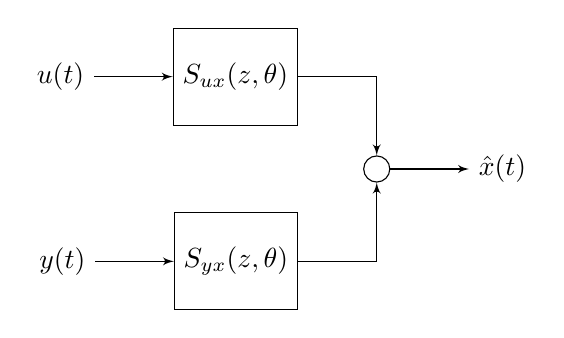
\begin{tikzpicture}[node distance=1cm,auto,>=latex']
\node (u) [] {$u(t)$};
\node (su) [right=of u,block] {$S_{ux}(z,\theta)$};
\node (ut) [right=of su,coordinate]{};
\node (add) [below=of ut,add]{};
\node (x) [right=of add]{$\hat{x}(t)$};
\node (yt) [below=of add,coordinate]{};
\node (sy) [left=of yt,block]{$S_{yx}(z,\theta)$};
\node (y) [left=of sy]{$y(t)$};
\path[->]
	(u) edge (su)
	(ut) edge (add)
	(add) edge (x)
	(y) edge (sy)
	(yt) edge (add);
\path[-]
	(su) edge (ut)
	(sy) edge (yt);
\end{tikzpicture}
\end{figure}
\subparagraph{Performance index}
\[
J_N(\theta)=
\frac{1}{N}\sum_{t=1}^N \left(
x(t)-(
	S_{ux}(z,\theta)u(t)+
	S_{yx}(z,\theta)y(t)
	)
\right)^2
\]
\subparagraph{Optimization}
\[
\hat{\theta}_N=\arg \min_\theta J_N(\theta)
\]
We get $S_{ux}(z,\hat{\theta}_N)$ and $S_{yx}(z,\hat{\theta}_N)$, the transfer functions for our software sensors

\section{Non-linear systems}
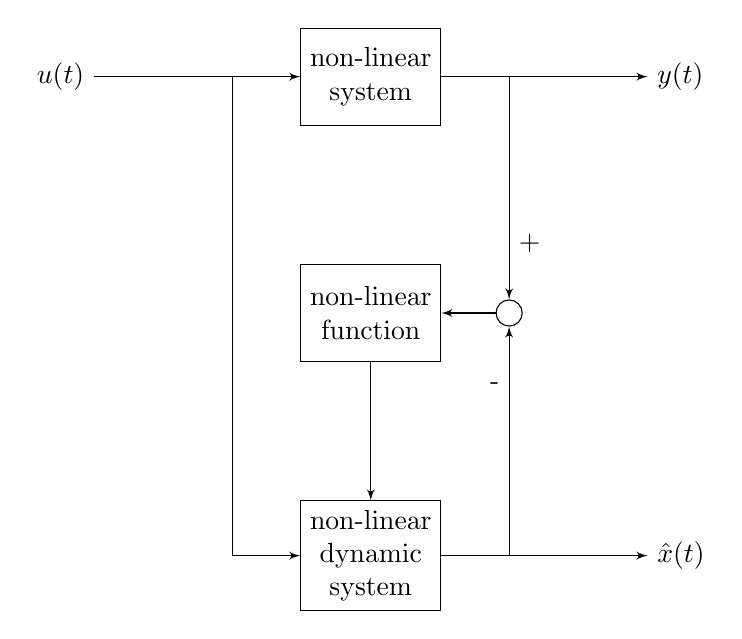
\begin{tikzpicture}[node distance=5em,auto,>=latex']
    \node (u) [] {$u(t)$};
    \node (ud) [right=of u,coordinate]{};
    \node [right of=ud,block,align=center] (sys) {non-linear\\system};
    \node (yd) [right of=sys,coordinate]{};
    \node (y) [right=of yd]{$y(t)$};
    \node (K) [below=of sys,block,align=center]{non-linear\\function};
    \node (add) [right of=K,add]{};
    \node (mod) [below=of K,block,align=center]{non-linear\\ dynamic\\ system};
    \node (ut) [left of=mod,coordinate]{};
    \node (xd) [right of=mod,coordinate]{};
    \node (x) [right=of xd]{$\hat{x}(t)$};
    \path[->]
    		(ud) edge (sys)
    		(yd) edge (y)
    		(yd) edge node[near end]{+}(add) 
    		(add) edge (K)
    		(K) edge (mod)
    		(ut) edge (mod)
    		(xd) edge node[near end]{-}(add)
    		(xd) edge (x);
    	\path[-]
    		(sys) edge (yd)
    		(u) edge (ud)
    		(ud) edge (ut)
    		(mod) edge (xd);
\end{tikzpicture}
\paragraph{Model}
\begin{center}
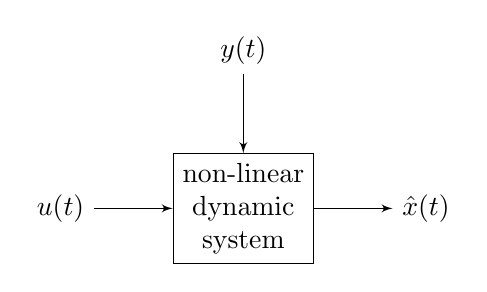
\begin{tikzpicture}[node distance=1cm,auto,>=latex']
\node (f) [block,align=center] {non-linear\\ dynamic\\ system};
\node (u) [left =of f] {$u(t)$};
\node (y) [above =of f] {$y(t)$};
\node (x) [right =of f]{$\hat{x}(t)$};
\path[->]
	(u) edge (f)
	(y) edge (f)
	(f) edge (x);
\end{tikzpicture}
\end{center}

\subsection{Recurrent neural network}
\begin{center}
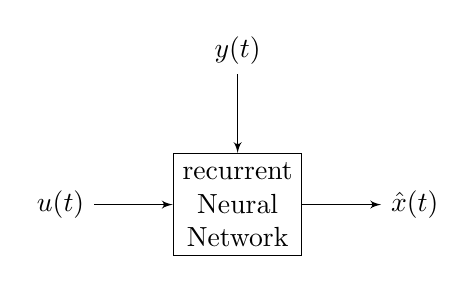
\begin{tikzpicture}[node distance=1cm,auto,>=latex']
\node (f) [block,align=center] {recurrent\\ Neural\\Network};
\node (u) [left =of f] {$u(t)$};
\node (y) [above =of f] {$y(t)$};
\node (x) [right =of f]{$\hat{x}(t)$};
\path[->]
	(u) edge (f)
	(y) edge (f)
	(f) edge (x);
\end{tikzpicture}
\end{center}
\subsection{FIR architecture} split the system into a static non-linear system and linear dynamics
\begin{center}
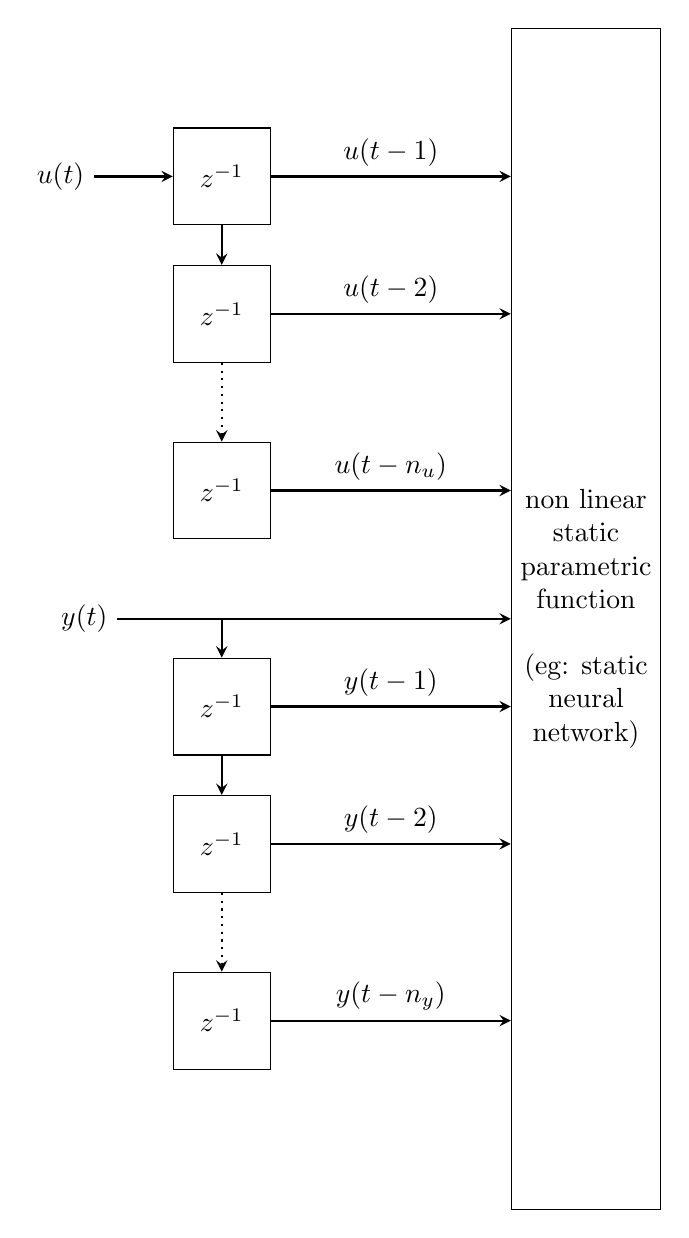
\begin{tikzpicture}[node distance=1cm,auto,>=latex']
\node (u) [] {$u(t)$};
\node (u1) [right =of u, block] {$z^{-1}$};
\node (u2) [below =.5 of u1, block] {$z^{-1}$};
\node (u3) [below =of u2, block] {$z^{-1}$};
\node (y1) [below =1.5 of u3, block] {$z^{-1}$};
\node (y) [below left = of u3]{$y(t)$};
\node (y2) [below =.5 of y1, block] {$z^{-1}$};
\node (y3) [below =of y2, block] {$z^{-1}$};
\node (sys) [block,right=5 of y,minimum height=15cm,align=center]{non linear \\ static \\ parametric \\ function\\\\(eg: static\\neural\\network)};
\draw[arrow] (u) -- (u1);
\draw[arrow] (u1) -- (u2);
\draw[arrow,dotted] (u2) -- (u3);
\draw[arrow] (u1) -- node[midway]{$u(t-1)$} (u1-|sys.west);
\draw[arrow] (u2) -- node[midway]{$u(t-2)$} (u2-|sys.west);
\draw[arrow] (u3) -- node[midway]{$u(t-n_u)$} (u3-|sys.west);
\draw[arrow] (y) -| (y1);
\draw[arrow]	(y) -- (sys);
\draw[arrow]	(y1) -- (y2);
\draw[arrow,dotted]	(y2) -- (y3);
\draw[arrow] (y1) -- node[midway]{$y(t-1)$} (y1-|sys.west);
\draw[arrow] (y2) -- node[midway]{$y(t-2)$} (y2-|sys.west);
\draw[arrow] (y3) -- node[midway]{$y(t-n_y)$} (y3-|sys.west);
\end{tikzpicture}
\end{center}
\subsection{IRR scheme}
\begin{center}
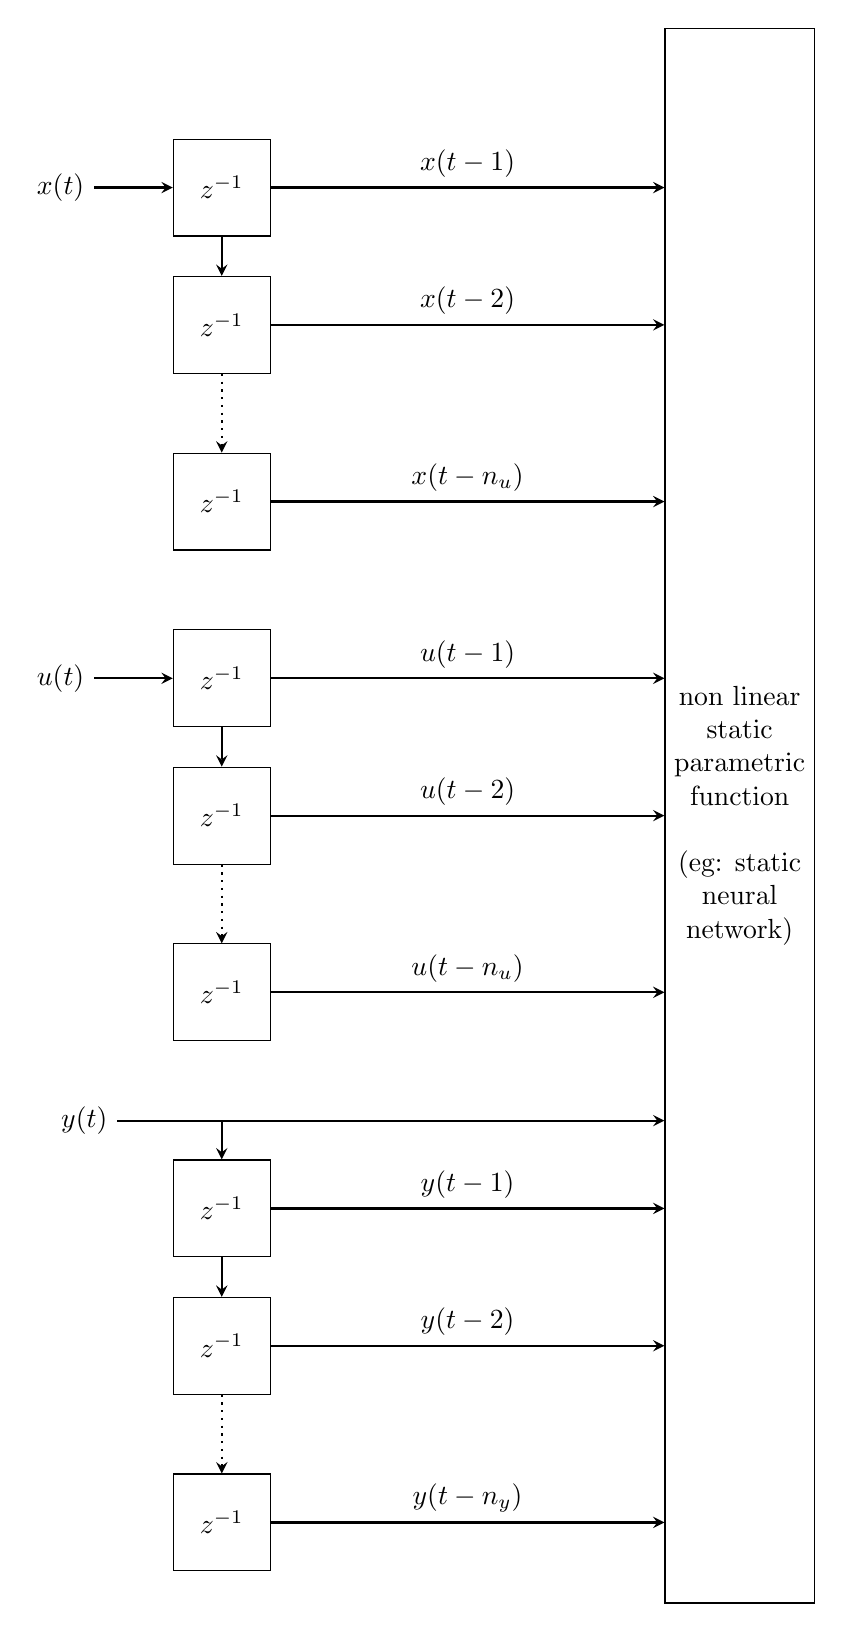
\begin{tikzpicture}[node distance=1cm,auto,>=latex']
\node (x) [] {$x(t)$};
\node (x1) [right=of x,block] {$z^{-1}$};
\node (x2) [below=.5 of x1,block] {$z^{-1}$};
\node (x3) [below=of x2,block] {$z^{-1}$};

\node (u1) [below=of x3, block] {$z^{-1}$};
\node (u) [left=of u1] {$u(t)$};
\node (u2) [below =.5 of u1, block] {$z^{-1}$};
\node (u3) [below =of u2, block] {$z^{-1}$};

\node (y1) [below =1.5 of u3, block] {$z^{-1}$};
\node (y) [below left = of u3]{$y(t)$};
\node (y2) [below =.5 of y1, block] {$z^{-1}$};
\node (y3) [below =of y2, block] {$z^{-1}$};

\node (sys) [block,right=5 of u2,minimum height=20cm,align=center]{non linear \\ static \\ parametric \\ function\\\\(eg: static\\neural\\network)};

\draw[arrow] (x)--(x1.west);
\draw[arrow] (x1)--(x2);
\draw[arrow,dotted] (x2)--(x3);
\draw[arrow] (x1)--node[midway]{$x(t-1)$}(x1-|sys.west);
\draw[arrow] (x2)--node[midway]{$x(t-2)$}(x2-|sys.west);
\draw[arrow] (x3) -- node[midway]{$x(t-n_u)$} (x3-|sys.west);

\draw[arrow] (u) -- (u1);
\draw[arrow] (u1) -- (u2);
\draw[arrow,dotted] (u2) -- (u3);
\draw[arrow] (u1) -- node[midway]{$u(t-1)$} (u1-|sys.west);
\draw[arrow] (u2) -- node[midway]{$u(t-2)$} (u2-|sys.west);
\draw[arrow] (u3) -- node[midway]{$u(t-n_u)$} (u3-|sys.west);

\draw[arrow] (y) -| (y1);
\draw[arrow]	(y) -- (y-|sys.west);
\draw[arrow]	(y1) -- (y2);
\draw[arrow,dotted]	(y2) -- (y3);
\draw[arrow] (y1) -- node[midway]{$y(t-1)$} (y1-|sys.west);
\draw[arrow] (y2) -- node[midway]{$y(t-2)$} (y2-|sys.west);
\draw[arrow] (y3) -- node[midway]{$y(t-n_y)$} (y3-|sys.west);
\end{tikzpicture}
\end{center}
\subsection{Physical regressors}
Using the physical knowledge of the system, provide a set of regressors (ie: smaller and more meaningful set of signals) elaborated by a static non-linear system
\begin{center}
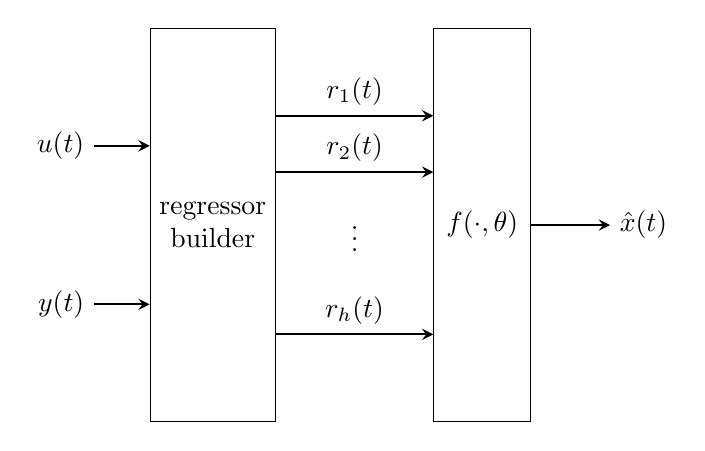
\begin{tikzpicture}[node distance=1cm,auto,>=latex']
\node (b1) [block,minimum height=5cm,align=center]{regressor\\builder};
\node (u) [above left = of b1.west] {$u(t)$};
\draw[arrow] (u) -- (u-|b1.west);
\node (y) [below left=of b1.west]{$y(t)$};
\draw[arrow] (y)--(y-|b1.west);
\node (b2) [block,minimum height=5cm,align=center,
right= 2 of b1]{$f(\cdot,\theta)$};
\draw[arrow] (b1.60) -- node[midway]{$r_1(t)$} (b1.60-|b2.west);
\draw[arrow] (b1.40) -- node[midway]{$r_2(t)$} (b1.40-|b2.west);
\draw[draw=none] (b1.-30) -- node[midway]{$\vdots$} (b1.-30-|b2.west);
\draw[arrow] (b1.-60) -- node[midway]{$r_h(t)$} (b1.-60-|b2.west);


\node(x) [right=of b2]{$\hat{x}(t)$};
\draw[arrow] (b2.east|-x)--(x);

\end{tikzpicture}
\end{center}

\part{Grey-box System Identification}
\section{Using Kalman Filter}
\subsection{Problem definition}
\begin{itemize}
\item We have a model:
\[
S:
\begin{cases}
x(t+1)=f(x(t),u(t),\theta)+v_1(t)\\
y(t)=h(x(t),\theta)+v_2(t)
\end{cases}
\]
\item $f$ and $h$ are functions (linear or not) depending on some unknown parameter $\theta$ carrying physical meaning (mass, resistance,...)
\item We want to estimate $\hat{\theta}$
\item This is archieved by managing the unknown parameters as extended states
\end{itemize}
\subsection{State extension}
\[
S:\begin{cases}
x(t+1)=f(x(t),u(t),\theta(t))+v_1(t)\\
\theta(t+1)=\theta(t)+v_\theta(t)\\
y(t)=h(x(t),\theta(t))+v_2(t)
\end{cases}
\]
And the extended state vector is $x_E=\begin{bmatrix}
x(t)\\\theta(t)
\end{bmatrix}
$\\
The noise in the equation of $\theta$ is added to prevent the KF form getting stuck on the initial conditions.
\subsection{Design choice} The choice of the covariance matrix of $v_\theta\sim WN(0,V_\theta)$\\
\begin{itemize}
\item Assume $v_1\perp v_\theta$ and $v_2\perp v_\theta$:
\[
V_\theta=\begin{bmatrix}
\lambda_{1\theta}^2\\
&\lambda_{2\theta}^2\\
&&\ddots\\
&&&\lambda_{n_\theta \theta}^2
\end{bmatrix}_{n_\theta \times n_\theta}
\]
\item Usually, it is assumed that $\lambda_{i\theta}=\lambda_{j\theta} \quad \forall i \forall j$
\item Assume that $v_\theta(t)$ is a set of \underline{independent} $WN$ all with the same variance $\lambda_\theta^2$
\item Bigger values of $\lambda_\theta^2$ lead to a quicker convergence, but less stable (stronger obscillations around the steady-state)
\item The selection of $\lambda_\theta^2$ is leaded by application-specific constraints
\end{itemize}
\subsection{Applicability} In theory, this trick can work with any number of sensors, states, and parameters. In practice it works well only on a limited number of parameters ($\sim$3 sensors, 5 states, 2 parameters)

\section{Simulation Error Method}
\begin{center}
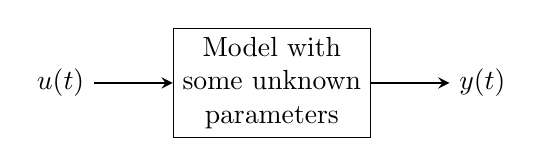
\begin{tikzpicture}[node distance=1cm,auto,>=latex']
\node (u) []{$u(t)$};
\node (mod) [right=of u,block,align=center]{Model with\\some unknown\\parameters};
\node (y) [right=of mod]{$y(t)$};
\draw[arrow] (u)--(mod);
\draw[arrow] (mod)--(y);
\end{tikzpicture}
\end{center}
\subsection{Dataset} from an experiment, collect:
\begin{align*}
\{\overline{u}(1),\overline{u}(2),\dots,\overline{u}(N)\\
\{\overline{y}(1),\overline{y}(2),\dots,\overline{y}(N)
\end{align*}
\subsection{Model}
\[
y(t)=\mathcal{M}(u(t),\overline{\theta},\theta)
\]
$\overline{\theta}$ is the set of known parameters, $\theta$ the set of unknown parameters
\subsection{Performance index}
\[
J_N(\theta)=\frac{1}{N}
\sum_{t=1}^N
\left(
\overline{y}(t)
-
\mathcal{M}(\overline{u}(t),\overline{\theta},\theta)
\right)^2
\]
\subsection{Optimization}
\[
\hat{\theta}_N=\arg\min_\theta J_N(\theta)
\]
\subsection{Limitations}
\begin{itemize}
\item Usually $J_N$ has no analytic expression
\item Computing the value of $J_N$ requires an entire simulation from $t=1$ to $t=N$
\item Usually $J_N$ is non-quadratic and non-convex $\rightarrow$ iterative and randomizad optimization must be used
\item Computationally demanding
\end{itemize}
\begin{center}
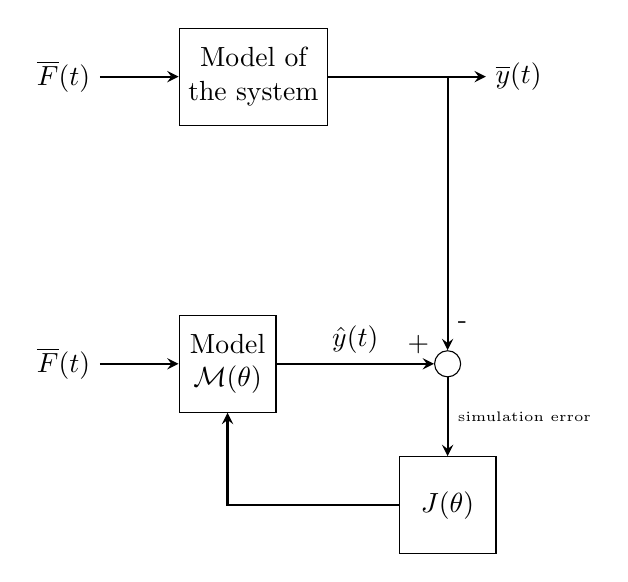
\begin{tikzpicture}[node distance=1cm,auto,>=latex']
\node (F1) [] {$\overline{F}(t)$};
\node (sysmod) [right=of F1,block,align=center] {Model of \\ the system};
\node (y) [right=2 of sysmod]{$\overline{y}(t)$};
\node (F2) [below=3 of F1]{$\overline{F}(t)$};
\node (mod) [right=of F2,block,align=center]{Model\\$\mathcal{M}(\theta)$};
\node (add) [right=2 of mod,add]{};
\node (J) [below=of add,block]{$J(\theta)$};
\draw[arrow] (F1)--(sysmod);
\draw[arrow] (sysmod)--(y);
\draw[arrow] (sysmod)-|node[pos=.95]{-}(add);
\draw[arrow] (F2)--(mod);
\draw[arrow] (mod)--node[midway]{$\hat{y}(t)$} node[pos=.90]{+} (add);
\draw[arrow] (add)--node[midway]{\tiny simulation error}(J);
\draw[arrow] (J)-|(mod);
\end{tikzpicture}
\end{center}

\part{Minimum Variance Control}
The goal is to design a feedback system
\begin{itemize}
\item Control design is the ain motivation of system identification and software sensing
\item MVC is based on prediction theory
\end{itemize}
\section{Setup the problem}
Consider a generic ARMAX model:
\[
y(t)=\frac{B(z)}{A(z)}u(t-k)
+\frac{C(z)}{A(z)}e(t)
\qquad
e(t)\sim WN(0,\lambda^2)
\]
\begin{align*}
B(z)&=b_0+b_1z^{-1}+\dots+b_pz^{-p}\\
A(z)&=1+a_1z^{-1}+\dots+a_mz^{-m}\\
C(z)&=1+c_1z^{-1}+\dots+c_nz^{-n}
\end{align*}
\paragraph{Assumptions}
\begin{itemize}
\item $\frac{C(z)}{A(z)}$ is in canonical form
\item $b_0\neq 0 \rightarrow$ k is the actual delay
\item $\frac{B(z)}{A(z)}$ is minimum phase $\iff$ all the roots of $B(z)$ are strictly inside the unit circle
\item $y^0(t)\perp e(t)$
\item $y^0(t)$ is known only up to the present time ($y^0(t)$ is totally unpredictable)
\end{itemize}
We want to determine the optimal tracking of the desired output behaviour:
\begin{center}
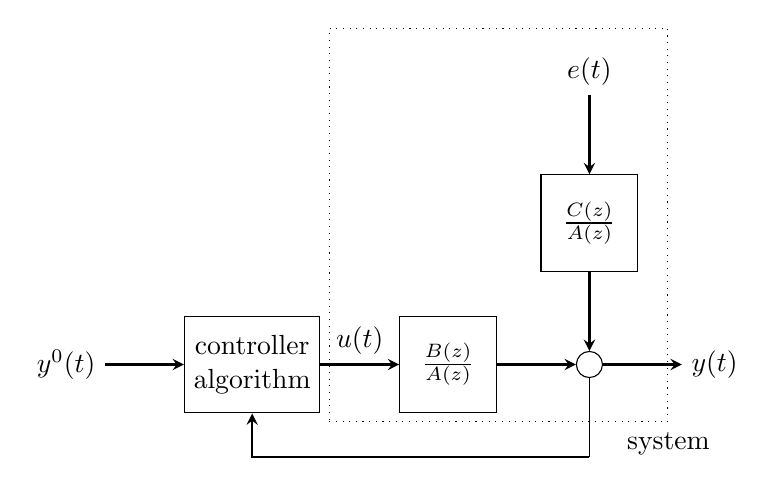
\begin{tikzpicture}[node distance=1cm,auto,>=latex']
\node (y0) [] {$y^0(t)$};
\node (cont) [block, right=of y0, align=center] {controller\\algorithm};
\node (Wu) [block, right=of cont]{$\frac{B(z)}{A(z)}$};
\node (add) [add, right=of Wu]{};
\node (We) [block,above=of add]{$\frac{C(z)}{A(z)}$};
\node (e) [above=of We]{$e(t)$};
\node (feed) [below = 1 of add, coordinate]{};
\node (y) [right=of add]{$y(t)$};
\draw[draw=none] (feed)--node[draw,rectangle,dotted,midway,
		minimum width=4.3cm,
		minimum height=5cm,
 		]{} node[below]{system}(y.south east);
\draw[arrow] (y0)--(cont);
\draw[arrow] (cont)--node[midway]{$u(t)$}(Wu);
\draw[arrow] (Wu)--(add);
\draw[arrow] (We)--(add);
\draw[arrow] (e)--(We);
\draw[arrow] (add)--(y);
\draw (add)--(feed);
\draw[arrow] (feed)-|(cont);
\end{tikzpicture}
\end{center}
Formally, MVC tries to minimize the following performance index:
\[
J=E\left[(y(t)-y^0(t))^2\right)
\]
Which is the variance of the tracking error
\subsection{Simplified problem 1}
\[
S:y(t)=ay(t-1)+b_0u(t-1)+b_1u(t-2)
\qquad
y(t)=\frac{b_0+b_1z^{-1}}{1-az^{-1}}u(t-1)
\]
Assuming:
\begin{itemize}
\item $y^0(t)=\overline{y}^0$
\item no noise
\item $b_0\neq 0$
\item Root of numerator inside the unit circle
\end{itemize}
\begin{align*}
J&=\left(y(t)-y^0(y)\right)^2\\
&=\left(y(t)-\overline{y}^0\right)^2\\
&=\left(ay(t-1)+b_0u(t-1)+b_1u(t-2)-\overline{y^0}\right)^2\\
&=\left(ay(t)+b_0u(t)+b_1u(t-1)-\overline{y^0}\right)^2\\
\frac{\delta J}{\delta u(t)}&=2\left(ay(t)+b_0u(t)+b_1\underbrace{u(t-1)}_{\substack{\text{number}\\\text{not variable}}}-\overline{y^0}\right)(b_0)
\end{align*}
\[
\frac{\delta J}{\delta u(t)}=0
\implies
ay(t)+b_0u(t)+b_1u(t-1)-\overline{y^0}=0
\implies
u(t)=(\overline{y}^0-ay(t))\frac{1}{b_0+b_1z^{-1}}
\]
\subsection{Simplified problem 2}
\[
S:y(t)=ay(t-1)+b_0u(t-1)+b_1u(t-2)+e(t)
\qquad
e(t)\sim WN(0,\lambda^2)
\]
\paragraph{Reference variable} $y^0(t)$
\paragraph{Performance index} $E\left[(y(t)-y^0(t))^2\right]$
\paragraph{Trick} rewrite $y(t)$ as
\[
y(t)=\hat{y}(t|t-1)+\epsilon(t)
\]
\[
k=1 
\implies \epsilon(t)=e(t) 
\implies y(t)=\hat{y}(t|t-1)+e(t)
\]
\begin{align*}
J&=E\left[\left(\hat{y}(t|t-1)+e(t)-y^0(t)\right)^2\right]\\
&=E\left[\left((\hat{y}(t|t-1)-y^0(t))+e(t)\right)^2\right]\\
&=E\left[\left(\hat{y}(t|t-1)-y^0(t)\right)^2\right]
+E\left[e(t)^2\right]
+\cancel{
2E\left[e(t)(\hat{y}(t|t-1)-y^0(t))\right]
}\\
\end{align*}
\[
\arg \min_{y^0(t)} E\left[\left(\hat{y}(t|t-1)-y^0(t)\right)^2\right]
+E\left[e(t)^2\right]
=
\arg \min_{y^0(t)} E\left[\left(\hat{y}(t|t-1)-y^0(t)\right)^2\right]
\]
The best result is when $\hat{y}(t|t-1)=y^0(t)$. Writing the system in terms of transfer functions we get:
\[
S:y(t)=
\frac{b_0+b_1z^{-1}}{1-az^{-1}}
u(t-1)
+
\frac{1}{1-az^{-1}}e(t)
\]
Applying the general 1-step predictor for $ARMAX$:
\[
\hat{y}(t|t-1)=\frac{b_0+b_1z^{-1}}{1}u(t-1)
+
\frac{1-1+az^{-1}}{1}y(t)
=
(b_0b_1z^{-1})u(t-1)+ay(t-1)
\]
Imposing the optimality condition we get:
\begin{align*}
b_0u(t-1)+b_1u(t-2)+ay(t-1)&=y^0(t)\\
b_0u(t)+b_1u(t-1)+ay(t)&=y^0(t+1)\\
u(t)&=\left(y^0(t+1)-ay(t)\right)\frac{1}{b_0b_1z^{-1}}
\end{align*}
Since we cannot predict the future we must approximate:
\[
u(t)
\approx
\left(y^0(t)-ay(t)\right)
\frac{1}{b_0+b_1z^{-1}}
\]
\subsection{General solution}
\[
S:y(t)=
\frac{B(z)}{A(z)}u(t-k)+
\frac{C(z)}{A(z)}e(t)
\qquad
e(t)\sim WN(0,\lambda^2)
\]
\paragraph{Assumptions}
\begin{itemize}
\item $b_0\neq 0$
\item $B(z)$ has all roots inside the unit circle
\item $\frac{C(z)}{A(z)}$ is in canonical form
\item $y^0(t)\perp e(t)$
\item $y^0(t)$ is unpredictable
\end{itemize}
\paragraph{Trick} rewrite $y(t)=\hat{y}(t|t-k)+\epsilon(t)$
\begin{align*}
J&=E\left[\left(\hat{y}(t|t-k)+\epsilon(t)-y^0(t)\right)^2\right]\\
&=E\left[\left((\hat{y}(t|t-k)-y^0(t))+\epsilon(t)\right)^2\right]\\
&=E\left[\left(
\hat{y}(t|t-k)-y^0(t)\right)^2\right]
+E\left[\epsilon(t)^2\right]
+\cancel{2E\left[\epsilon(t)\left(\hat{y}(t|t-k)-y^0(t)\right)\right]}\\
&=E\left[\left(
\hat{y}(t|t-k)-y^0(t)\right)^2\right]+\textbf{constant}
\end{align*}

\part{Recursive Identification}
\section{Least square}
\[
\hat{\theta}_N=\arg\min_\theta
\left\lbrace
J_N(\theta)=
\frac{1}{N}\sum_{t=1}^{N}
\left(
y(t)-\hat{y}(t|t-1,\theta)
\right)^2
\right\rbrace
\]
We want to find the predictor model $\hat{y}(t|t-1,\theta)$
\[
y(t)=\phi(t)^T\theta+e(t)
\]
Since $e(t)$ is unpredictable, the best possible 1-step predictor is $\hat{y}(t|t-1,\theta)=\phi(t)^T\theta$. Substituting in $J$:
\[
J_N(\theta)=\frac{1}{N}
\sum_{t=1}^N
\left(y(t)-\phi(t)^T\theta\right)^2
\]
Analytically we can find the minimum:
\begin{align*}
\frac{\delta J_N(\theta)}{\delta \theta}&=0\\
\hat{\theta}_N&=S(N)^{-1}\sum_{t=1}^N \phi(t)y(t)\\
S(N)&=\sum_{t=1}^N \phi(t)\phi(t)^T
\end{align*}
But the procedure must be repeated at each $t$ step
\subsection{Recursive Least Square}
\begin{center}
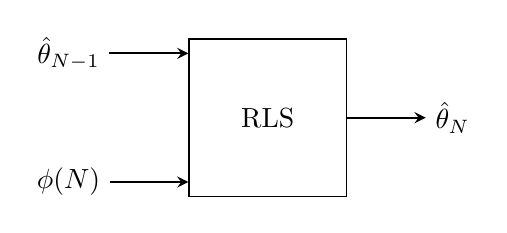
\begin{tikzpicture}[node distance=1cm,auto,>=latex']
\node (theta) [] {$\hat{\theta}_{N-1}$};
\node (phi) [below=of theta] {$\phi(N)$};
\coordinate (mid) at ($(theta.east)!0.5!(phi.east)$);
\node (RLS) [right=of mid,block,minimum height=2cm,minimum width=2cm]{RLS};
\node (res) [right=of RLS] {$\hat{\theta}_N$};
\draw[arrow] (theta)--(theta-|RLS.west);
\draw[arrow] (phi)--(phi-|RLS.west);
\draw[arrow] (RLS)--(res);
\end{tikzpicture}
\end{center}
\subsection{First form}
\begin{align*}
\hat{\theta}_N&=S(N)^{-1}\sum_{t=1}^N \phi(t)y(t)\\
S(N)\hat{\theta}_N&=\sum_{t=1}^N \phi(t)y(t)\\
S(N-1)\hat{\theta}_{N-1}&=\sum_{t=1}^{N-1} \phi(t)y(t)\\
\sum_{t=1}^N \phi(t)y(t)&=\sum_{t=1}^{N-1} \phi(t)y(t)+\phi(N)y(N)\\
\sum_{t=1}^N \phi(t)y(t)&=S(N-1)\hat{\theta}_{N-1}+\phi(N)y(N)\\
\Aboxed{
\hat{\theta}_N&=\hat{\theta}_{N-1}+S(N)^{-1}\phi(N)\left[y(N)-\phi(N)^T\hat{\theta}_{N-1}\right]
}\\
S(N)&=S(N-1)+\phi(N)\phi(N)^T
\end{align*}
However, this way $S(N)\to\infty$, so the domputing unit saturates.
\subsection{Second form} Normalize wrt. $N$
\begin{align*}
S(N)&=S(N-1)+\phi(N)\phi(N)^T\\
R(N)&=\frac{1}{N}S(N)\\
R(N)&=\frac{N-1}{N}R(N-1)+\frac{1}{N}\phi(N)\phi(N)^T\\
K(N)&=\frac{1}{N}R(N)^{-1}\phi(N)\\
\epsilon(N)&=y(N)-\phi(N)^T\hat{\theta}_{N-1}\\
\Aboxed{
\hat{\theta}_N&=\hat{\theta}_{N-1}+K(N)\epsilon(N)
}
\end{align*}
This however reqires matrix inversion at each iteration, which is expensive
\subsection{Third form} 
It can be proven that the following works
\begin{align*}
\epsilon(N)&=y(N)-\phi(N)^T\hat{\theta}_{N-1}\\
\Aboxed{
V(N)&=V(N-1)-
\frac{
	V(N-1)\phi(N)\phi(N)^TV(N-1)
}{
	1+\phi(N)^TV(N-1)\phi(N)
}
}\\
\Aboxed{
K(N)&=V(N)\phi(N)
}\\
\hat{\theta}_N&=\hat{\theta}_{N-1}+K(N)\epsilon(N)
\end{align*}
This does not require matrix inversion
\subsection{Forgetting factor}
If theta contains some parameter changing over time, the objective function should "forget" old data. The new objective function becomes:
\[
J_N(\theta)=\frac{1}{N}
\rho^{N-t}\left(\hat{y}(t|t-1,\theta)\right)^2
\]
Where $\rho\in\left[0,1\right]$ is the forgetting factor (the smaller, the more forgetful). The new equations become:
\begin{align*}
\epsilon(N)&=y(N)-\phi(N)^T\hat{\theta}_{N-1}\\
\Aboxed{
S(N)&=\rho S(N-1)+\phi(N)\phi(N)^T
}\\
K(N)&=S(N)^{-1}\phi(N)\\
\hat{\theta}_N&=\hat{\theta}_{N-1}+K(N)\epsilon(N)
\end{align*}

\newpage
\part{Cheatsheet}
\section{Probability Recall}
\paragraph{Cross-Variance}
$Var[v,u]=E[(v-E[v])(u-E[u])]$
\paragraph{Variance Matrix}
$\begin{vmatrix}
	Var[v_1]			&	.	&	.	&	Var[v_1,v_k]		\\
		.			&	.	&		&		.			\\
		.			&		&	.	&		.			\\
	Var[v_k,v_1]		&	.	&	.	&	Var[v_k]			\\
				
\end{vmatrix}$
\paragraph{Covariance coefficient}
	$\delta[i,j]=\frac{Var[i,j]}{\sqrt{Var[i]}\sqrt{Var[j]}}$
\paragraph{Stationary process}
\begin{itemize}
	\item $m$ constant
	\item $\lambda^2$ constant
	\item covariance $\gamma(\tau)$ depends only on time difference
	\item $|\gamma(\tau)|\leq\gamma(0)		\quad\forall\tau$
\end{itemize}
\paragraph{White noise} $\eta(t)\sim WN(m,\lambda^2)$
\begin{itemize}
	\item Stationary process
	\item $\gamma(\tau)=0	\quad\forall\tau\neq0$
	\item $v(t)=\alpha \eta (t)+\beta\implies v(t)\sim WN(\beta,\alpha^2 \lambda^2)$
\end{itemize}
\paragraph{Canonical representation}
\begin{itemize}
\item Monic
\item Same degree
\item Coprime
\item Poles and zeros in unit disk
\end{itemize}
\section{Spectral analysis}
\paragraph{Spectrum}
\begin{itemize}
\item $\Gamma(\omega)=\gamma(0)+2cos(\omega)\gamma(1)+2cos(2\omega)\gamma(2)+...$
\item Periodic $T=2\pi$
\item Even
\item $\Gamma_\eta(\omega)=\gamma_\eta(0)=\lambda^2$
\end{itemize}
\paragraph{Complex spectrum}
\begin{itemize}
\item $\Phi(z)=\sum_{\tau =-\infty}^{+\infty} \omega(\tau)z^{-\tau}$
\item $\Gamma(\omega)=\Phi(e^{j\omega})$
\end{itemize}
\paragraph{Fundamental theorem of spectral analysis}
\begin{itemize}
\item $\Gamma_{\text{out}}(\omega)=|W(e^{j\omega})|^2 \cdot \Gamma_{\text{in}}(\omega)$
\item $\Phi_{\text{out}}(z)=W(z)W(z^{-1}) \cdot \Phi_{\text{in}}(z)$
\end{itemize}
\section{Moving Average MA(n)}
\begin{itemize}
\item $W(z)=\frac{c_0z^n+c_1z^{n-1}+...+c_n}{z_n}$
\item $m=0$
\item $\gamma(\tau)= 
\begin{cases}
(c_0c_\tau+c_1c_{1+\tau}+...+c_{n-\tau}c_\tau)\lambda^2	&	|\tau|\leq n\\
0	& \text{otherwise}
\end{cases}$
\end{itemize}
\subsection{MA($\infty$)}
\begin{itemize}
\item $\gamma(0)=(c_0^2+c_1^2+...+c_k^2+...)\lambda^2$
\item $\gamma(0)$ must converge to a finite value
\end{itemize}
\section{Auto Regressive AR(n)}
\begin{itemize}
\item $m=0$
\item $W(z)=\frac{z^n}{z^n-a_1z_{n-1}-...-a_n}$
\item Covariance calculated by its definition
\end{itemize}

\section{Known predictors}
\begin{description}
\item[AR(1)] $\hat{v}(t|t-r)=a^rv(t-r)$
\item[MA(1)] $\hat{v}(t|t-1)=v(t-1)-c\hat{v}(t-1|t-2)$
\item[MA(n)] $\hat{v}(t|t-\textbf{k})=0 \quad \forall k>n$
\item[ARMA($n_a,n_b$)] $\hat{v}(t|t-1)=
\frac{C(z)-A(z)}{C(z)}v(t)$
\item[ARMAX($n_a,n_b$)] $\hat{y}(t|t-1)=
\frac{C(z)-A(z)}{C(z)}y(t)
+\frac{B(z)}{C(z)}u(t-1)$
\end{description}
\end{document}
